\documentclass{article}
\usepackage{graphicx}
\usepackage{hyperref}
\graphicspath{ {./images/} }
%Includes References in the table of contents%
\usepackage[nottoc]{tocbibind}
\usepackage{float}
\usepackage{amsmath}
\usepackage{pdfpages}

\usepackage[T1]{fontenc}
\usepackage[utf8]{inputenc}
\usepackage{authblk}

\usepackage[square, numbers]{natbib}
\bibliographystyle{abbrvnat}

\title{News article summarization}
\author{
  Günay, A\\
  \texttt{911443}
  \and
  Sormunen, T\\
  \texttt{878902}
  \and
  Vasileios, Christoforidis***\\
  \textbf{Couldn't be reached during project.\\ Only contributed to the project planning}
}
\renewcommand\Authands{ and }


\newcommand{\bertlarge}{$\text{BERT}_{LARGE}$ }
\newcommand{\bertbase}{$\text{BERT}_{BASE}$ }
\newcommand{\gptmedium}{$\text{GPT-2}_{MEDIUM}$ }
\newcommand{\gptlarge}{$\text{GPT-2}_{LARGE}$ }

% No need to use noindent all the time :D
\setlength\parindent{0pt}

\begin{document}
	
\maketitle

\begin{abstract}
	\noindent
	In our project, we have decided to create text summarizer with BERT. 
	There is already a Bert Extractive Summarizer -package. It's based on following article: \href{https://arxiv.org/ftp/arxiv/papers/1906/1906.04165.pdf}{https://arxiv.org/ftp/arxiv/papers/1906/1906.04165.pdf}
	This package is intended for lecture-summarization, and our goal is to extend and fine-tune this model for news or scientific articles.
	Even though foundational work is already done for the package, there's still much to customize such as tokenizer and model. 
	Our target language is english. Summarization tools such as Bilingual Evaluation Understudy (BLEU) and Recall-Oriented Understudy for Gisting Evaluation (ROUGE) are available, and part of the project is to try to evaluate the texts automatically and manually.	
\end{abstract}

\clearpage
\section{Introduction}

Automatic summarization is the process of shortening a set of data computationally, to create a subset (a summary) that represents the most important or relevant information within the original content. There are two main approaches to automatic summarization (independently of the application domain, e.g. text, images, video etc.):
\begin{itemize}
	\item Extraction-based or extractive summarization 
	\item Abstraction-based or abstractive summarization
\end{itemize}

When it comes to text documents, summarization is closely related to data compression and information understanding. The ability to produce coherent, well-structured summaries has the potential to transform efficiently the way that discovery systems work, as well as help human readers in skimming large datasets of text documents. That is why automatic summarization is considered one of the most important, yet least solved, tasks in NLP and a method that will transform the way people consume information on the Internet. In conclusion, applying text summarization reduces reading time, accelerates information retrieval and increases the amount of useful, dense information. In our case, we will deal with extractive summarization where a system produces summaries by choosing a subset of the initial text.

\clearpage
\section{Background}
The first summarization techniques go back already more than 50 years to Luhn’s and Edmundson’s seminal papers on automatic summarization (1958 and 1969 respectively, \cite{textmining1958}, \cite{automaticextracting}). Early work in the field dealt with single document summarization (news story, scientific articles etc.) Later, multi document summarization was applied in big data clusters to provide a coherent and brief digest to the users. \\

In work by \cite{extractive_bert} they investigated a new way for creating extractive summaries for lectures. They tested K-means clustering for high dimensional embeddings produced from different deep learning models (BERT, GPT-2) and their ensembles. Here the K-hyperparameter represents the amount of sentences that are used in the summary. Idea was, that by finding different clusterings of the embeddings it would be possible to find different types of sentences in different clusters. Then from these clusters, they would take the most central sentence and use it in the summary. 


\clearpage
\section{Methods}

In many NLP tasks, the shortage of training data is often the source of the problems. There has been some research to tackle this issue by using unannotated text on the internet for training language representation models that serve general purpose. This process is also known as pre-training. The idea is that the pre-trained model can be fine-tuned later on small-data NLP tasks like question answering and sentiment analysis to have significant accuracy improvements compared to training on these datasets from scratch. 

In our project, we mainly used GPT-based and BERT-based pre-trained models for text summarization.

\subsection*{GPT}

GPT, also known as Generative Pre-trained Transformer, is the first semi-supervised approach to language models. The procedure is to train a generative language model using unlabeled data and fine-tune the model with examples of NLP tasks like sentiment analysis, textual entailment and question answering. The goal is to learn a universal representation that transfers with little adaptation to a wide range of tasks. \\

The training is in two stages: first, using a language modeling objective on unlabeled data to learn the initial parameters of a neural network mode then adapting these parameters to a target task using the supervised objective. The data set used in training is BooksCorpus which includes over 7,000 unique unpublished books from a variety of genres and especially, long sections of continuous text that allows the model to learn to handle long-range dependencies in the text. \cite{bookscorpus}\\

For the model architecture, GPT uses transformers which have been shown to perform strongly on various NLP tasks such as machine translation and document generation. Transformers allow the model to have a better structured memory for dealing with long-term dependencies in the text, compared to other methods like recurrent neural networks which are not able to preserve these dependencies well. Below figure about the model architecture is taken from the original paper.

\begin{figure}[H]
	\centering
	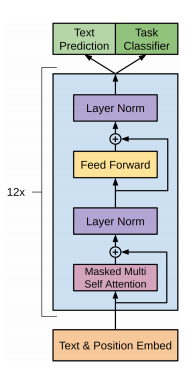
\includegraphics[scale=0.65]{reports/Final report/images/gpt_model.png}
	\caption{Model architecture of GPT}
	\label{fig:gpt}
\end{figure}


\subsection*{BERT }

BERT, also known as Bidirectional Encoder Representations from Transformers, is an example of pre-trained language representation models which uses a combination of masked language modeling objective and next sentence prediction on a large plain text corpus including Wikipedia and the Toronto Book Corpus. Unlike other language representation models, BERT is designed bidirectional in the way that it reads the input sequences. This characteristic allows the model to learn the context of a word from both left and right sides, capturing the previous and next contexts. BERT can also be fine tuned with one additional output layer to create state-of-the-art models for a wide range of tasks, such as question answering and language inference, without substantial task-specific architecture modifications. \cite{devlin2019bert}

\begin{figure}[h]
	\centering
	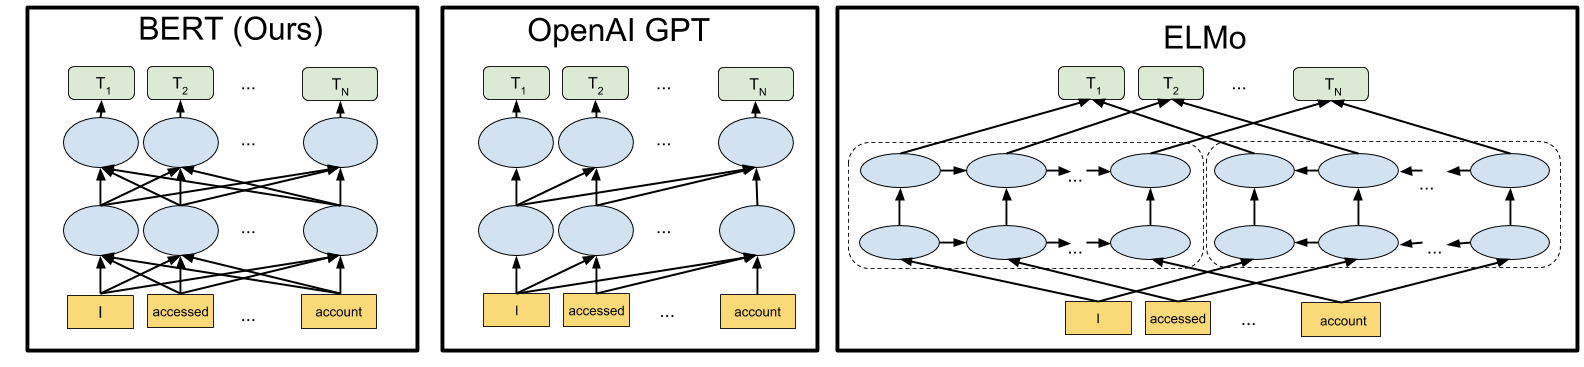
\includegraphics[scale=0.2]{bert.png}
	\caption{Architectures of known pre-training methods}
	\label{fig:mesh1}
\end{figure}

In the above figure created by Google AI, the neural network architectures state-of-the-art contextual pre-training methods are shown. The arrows show the information flow through layers while the green boxes indicate the final contextualized representation for input words. It can be seen that BERT is deeply bidirectional while OpenAI's GPT is unidirectional and ELMo has a shallow bidirectional structure.

BERT can also be considered conceptually simple. As mentioned earlier, BERT uses the advantage of bidirectionality by using a masked language modeling objective. Some words in the input text are masked out and each word are conditioned bidirectionally to predict the those masked words. It also uses next sentence prediction in which the model predicts if a sentence logically follows another sentence which was given previously. This task enables BERT to capture the relationship between sentences. \cite{devlin2019bert}

BERT has also been used in previous work for text summarization for news. In his paper, Yang suggests a fine tuned variant of BERT called BERTSUM for extractive summarization in which the input sequence and embeddings of BERT are modified to make it possible for extracting summaries. It is concluded that BERTSUM with inter-sentence Transformer layers achieve the best performance for extractive summarization of news, using CNN/DailyMail news and New York Times Annotated Corpus. \cite{liu2019finetune}


\subsection*{LEDE-3 }

LEDE-3 is a rule-based summarization strategy which copies the first sentence, first paragraph, or first \textit{n} words of the text to produce a summary. It is often used as a baseline in performance evaluation. In our project, we use LEDE-3 as the first three sentences of the news articles form the summary. Although the underlying idea is simple, this method is still competitive with state-of-the-art systems as the articles tend to have the most quality sentences in first sentence, first paragraph or a sequence. \cite{dataset}
\clearpage
\section{Experiments}

The underlying algorithm for \cite{extractive_bert} works as following: first, the sentence embeddings for text to be summarized are generated with selected model (BERT or GPT-2). On these embeddings, then K-means clustering algorithm is performed with pre-defined amount of clusters K. Each cluster center then clusters semantically similar sentences, and the algorithm takes the most central embedding in the respective cluster. The idea is that different clusters would find different type of sentences, and the most central sentence should represent the cluster the best.\\

K-hyperparameter should be chosen before the experiment is carried out. In this case K is chosen as a ratio for summarization sentence amount and original text sentence amount. In practise ratio of 0.5 would mean that we want to generate a summary that has half the amount of sentences that are in the original text to-be-summarized. In the experiments ratio of 0.2 was used. This might however be slightly too large for news articles, as we see from figures in Section 5. More appropriate ratio might be between 0.1 and 0.2, but 0.2 also provides sufficient results. \\

\clearpage
\section{Results}

Evaluation was done on newsroom dataset \cite{dataset}. The model inference however is extremely slow, and only a subset of samples was chosen to be evaluated. The sample size was chosen to be 500 at randomly, which resulted in tolerable running times ($<$ 60 minutes). Evaluations were automated, but also manual sanity checks were done. These sanity checks are however not listed here in the report, as it would take unnecessarily much space. \\

\subsection{General text properties}

\noindent
Two different BERT models were tested, \bertlarge and \bertbase. These models were compared against baseline model Lede-3 and GPT-2. GPT-2 was chosen to be compared against BERT models, because in the original study \cite{extractive_bert} they noticed that BERT should be generating more representative embeddings of the sentences. Also \gptlarge was chosen as one model to be evaluated. \gptlarge has 774 million parameters, which is roughly the double of parameters in \bertlarge and \gptmedium. Also GPT-2-XL and new GPT-NEO (GPT-3 replication) would've been interesting comparisons, but unfortunately they were too large to fit on GPU.\\

\noindent
The python package bert-extractive-summarizer \cite{extractive_bert} uses only sentences from original text, and the amount of sentences is defined by either fixed ratio, or amount of sentences. In this case the ratio was defaulted to 0.2, which means that we use 20\% of the sentences from original text. We can calculate empirical distribution of the ratios seen in reference summaries as displayed in Figure \ref{fig:empirical_ratio}.


\noindent
\begin{figure}[H]
	\centering
	\hspace*{-3cm}
	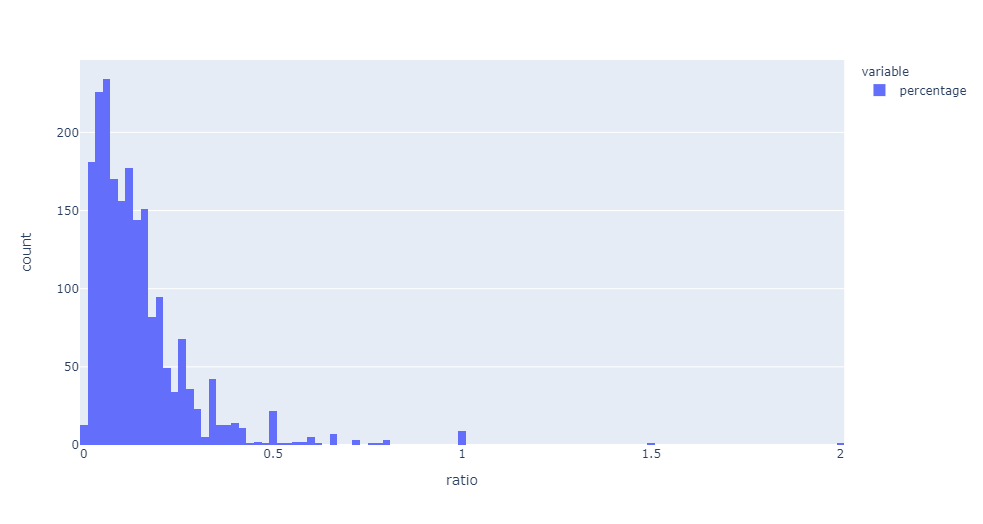
\includegraphics[scale=0.55]{empirical_ratio.png}
	\caption{Distribution of observed ratios in the data}
	\label{fig:empirical_ratio}
\end{figure}

\noindent
Here we can see that the mean is around 0.15. We can also plot how many sentences there are in summaries which is seen in Figure \ref{fig:empirical_lengths}.

\noindent
\begin{figure}[H]
	\centering
	\hspace*{-3cm}
	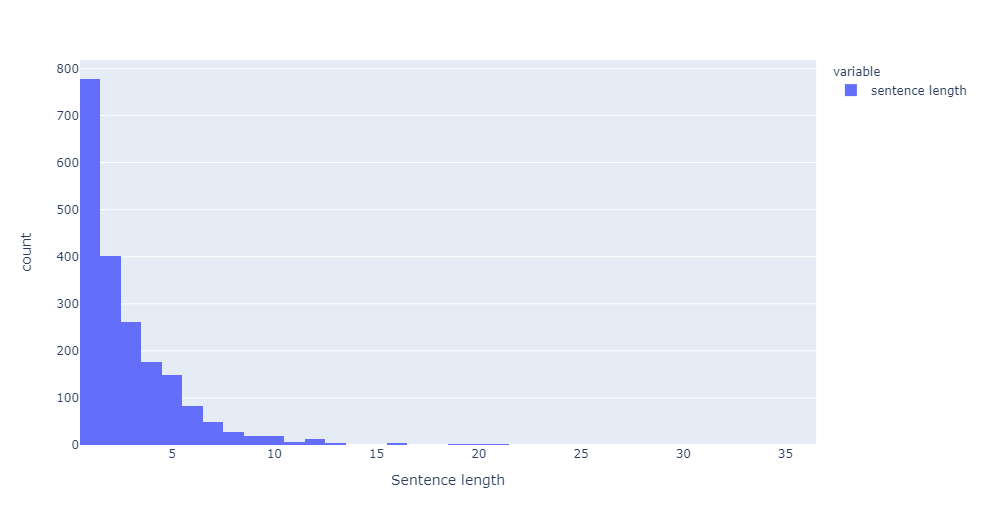
\includegraphics[scale=0.55]{empirical_lengths.png}
	\caption{Distribution of observed ratios in the data}
	\label{fig:empirical_lengths}
\end{figure}

\noindent
Here we actually see that there are multiple summaries which have sentence amount of 1. This is important to remember because it might favor Lede-3 classifier due to shortness of text, as we will see later.\\

\noindent
We can also view the true summary distribution statistics from the Newsroom-dataset website summari.es \cite{dataset}. By using their visualization tool, we get following distribution for amount of words in summaries. \\

\noindent
\begin{figure}[H]
	\centering
	\hspace*{-3cm}
	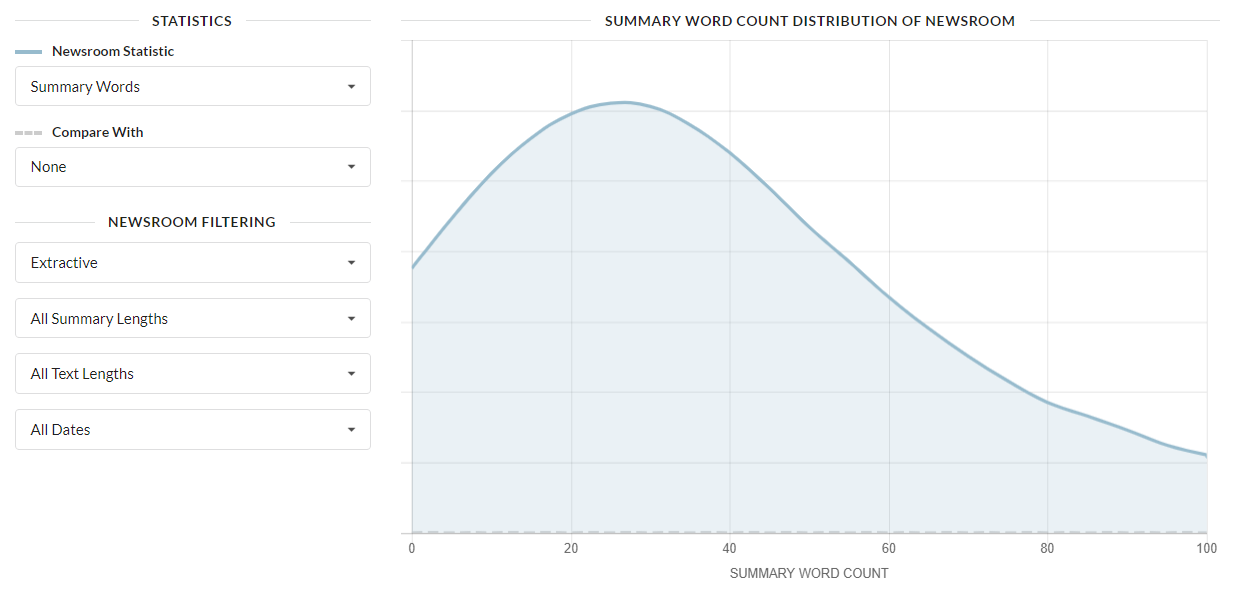
\includegraphics[scale=0.55]{words_in_summary.png}
	\caption{Distribution of words in summaries}
	\label{fig:words_in_summary}
\end{figure}

\noindent
To compare this distribution with our empirical distribution, we also need to plot summary word distribution. When we plot amount of words seen in our samples, we get similar looking plot to Figure \ref{fig:words_in_summary} in our new Figure \ref{fig:empirical_summary_words}.\\

\noindent
\begin{figure}[H]
	\centering
	\hspace*{-3cm}
	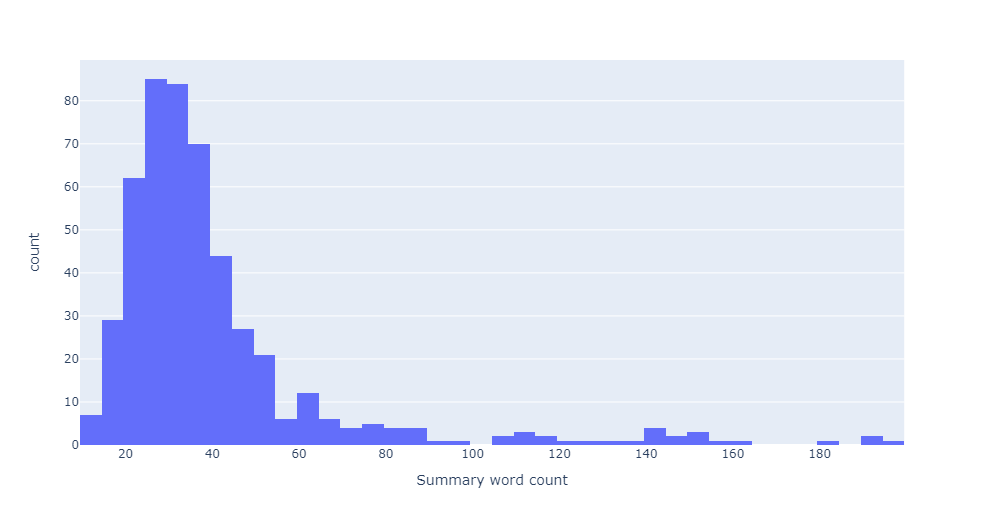
\includegraphics[scale=0.55]{empirical_summary_words.png}
	\caption{Distribution of words in summaries}
	\label{fig:empirical_summary_words}
\end{figure}

\noindent
This leads to a conclusion, that news article summaries are quite short in general. Because the word distribution for summaries matches, it also means that our Figure \ref{fig:empirical_lengths} describes the amount of sentences quite well.\\

\subsection{Recall-Oriented Understudy for Gisting Evaluation (Rouge)}

ROUGE is a metric which determines the quality of summary. In this experiment we used ROUGE-N and ROUGE-L metrics. ROUGE-N metric measures n-gram overlapping between generated and reference summaries. ROUGE-L metric compares the longest common subsequence between generated and reference summaries. ROUGE recall can be defined as following \cite{rouge}: \\

\begin{align*}
	\text{ROUGE-recall} &= \dfrac{\text{n-overlapping-words}}{\text{n-words-in-reference-summary}}
\end{align*}\\

\noindent
and ROUGE precision as following:\\

\begin{align*}
	\text{ROUGE-precision} &= \dfrac{\text{n-overlapping-words}}{\text{n-words-in-generated-summary}}
\end{align*}\\

\noindent
ROUGE-f1 score used in the coding implementation is similar to normal f1-scores, this time just used with ROUGE-precision and ROUGE-recall. \cite{rouge}\\

\noindent
Rouge scores seem to be dominated by Lede-3. Lede-3 is known to have strong performance, comparable with state-of-art methods as discussed in \cite{dataset}. Otherwise the models are performing similarly, although \gptmedium is achieving slightly higher scores. All of the rouge scores are seen in Figures \ref{fig:rouge1_02}, \ref{fig:rouge2_02} and \ref{fig:rougel_02} below. 

\begin{figure}[H]
	\centering
	\hspace*{-3cm}
	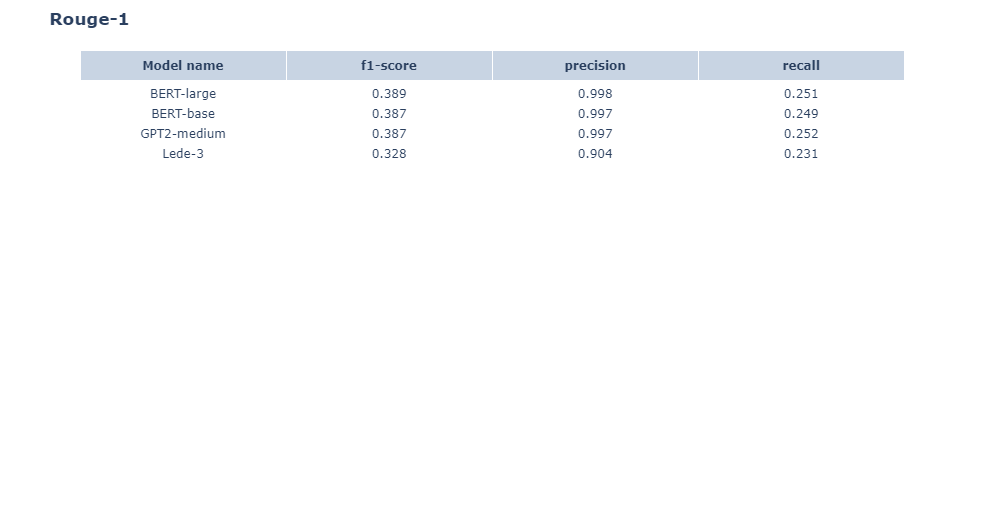
\includegraphics[scale=0.55]{rouge1.png}\\
	\caption{Rouge-1 scores with text-to-summary sentence-ratio=0.2}
	\label{fig:rouge1_02}
\end{figure}

\begin{figure}[H]
	\centering
	\hspace*{-3cm}
	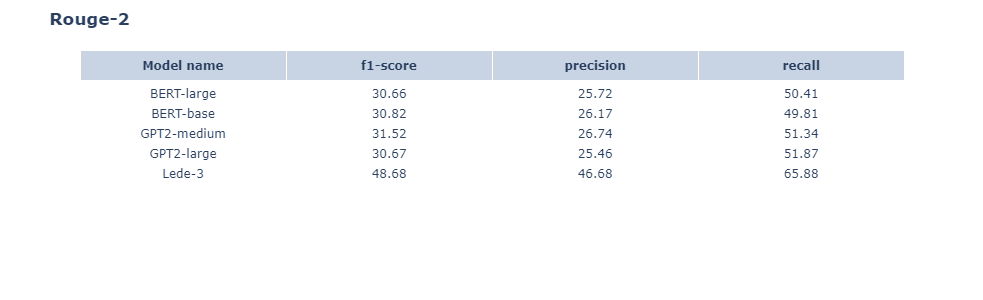
\includegraphics[scale=0.55]{rouge2.png}\\
	\caption{Rouge-2 scores with text-to-summary sentence-ratio=0.2}
	\label{fig:rouge2_02}
\end{figure}

\begin{figure}[H]
	\centering
	\hspace*{-3cm}
	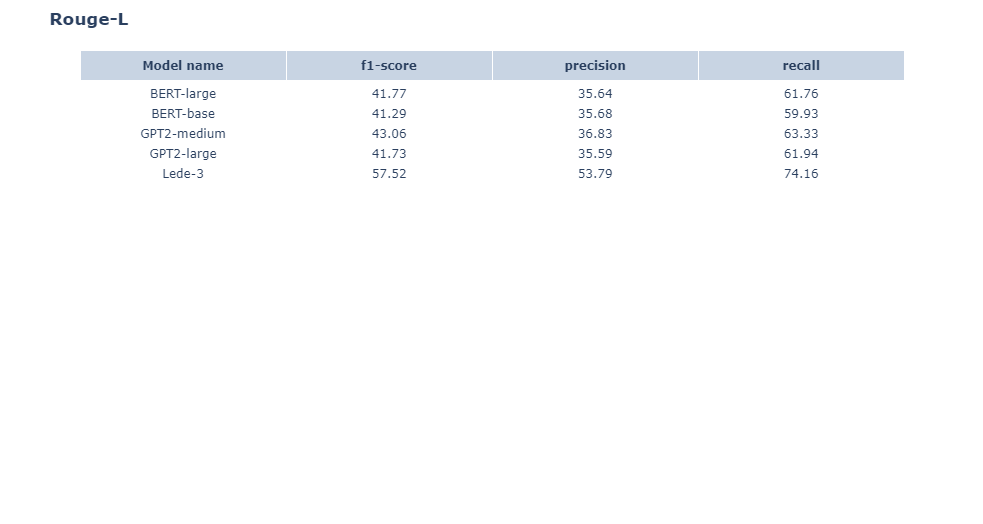
\includegraphics[scale=0.55]{rougel.png}\\
	\caption{Rouge-L scores with text-to-summary sentence-ratio=0.2}
	\label{fig:rougel_02}
\end{figure}

\subsection{Bilingual Evaluation Understudy (BLEU)}

\noindent
We can also take a look at BLEU scores for each model. BLEU measures how much the n-grams in our generated summary appears in the reference summaries. BLEU performs similarly to ROUGE-precision, except BLEU introduces brevity penalty, which penalizes generated summaries that are shorter than reference summaries. As Lede-3 summaries are always of length 3, in tasks where reference summaries are long, this would lead to penalizing Lede-3 model. In our case we can estimate how much Lede-3 is punished by looking at how many reference summaries have 3 sentences or more from the summary distribution in Figure \ref{fig:empirical_lengths}. We see that majority of the sentences are under length 3. This means that Lede-3 sentences are not punished, and it actually provides really good performance on this dataset as we see in Figure \ref{fig:bleu}. 

\begin{figure}[H]
	\centering
	\hspace*{-2cm}
	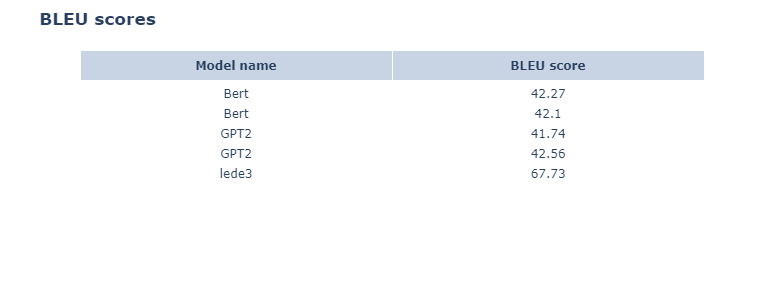
\includegraphics[scale=0.55]{bleu_scores.png}\\
	\caption{BLEU scores with 4-grams}
	\label{fig:bleu}
\end{figure}

\clearpage
\section{Discussion}

\noindent
In this experiment we saw how well extractive text summarization works if we choose sentences based on their centrality. We used K-means clustering to cluster embeddings that are achieved from models. Then we picked the most central embeddings of each cluster. We used Lede-3 as baseline, and also compared GPT-models to our BERT-model to see how well they produce embeddings. We found out that Lede-3 acually is the most accurate summarization technique in this sense. Although Lede-3 is very simple algorithm and it has no understanding of the underlying text, it seems like the texts are written in such way that first sentences produce most important aspects of the text. This is interesting realization, and in the future it would be interesting to try to fine tune some deep learning model to see, whether it actually is able to outperform Lede-3 or not.\\

\noindent
In this experiment it was also interesting to see how four state-of-art models performed when extracting embeddings without fine tuning. Most interesting note was that scaling the model (\gptlarge) didn't necessarily result in better embeddings with respect to our task.\\

\noindent
This clustering approach was used when summarizing lecture videos in \cite{extractive_bert}, where this approach is more viable because lectures aren't as well structured as news articles. 

\clearpage
\section{Division of labor}

The labor was divided between Günay and Sormunen. Günay was mostly responsible for the model write up and implementation, and Sormunen was responsible for the model evaluation and data pipeline production. Work was equally divided, and done in a good spirit. 

% Import bibliography file %
\bibliography{citations/sources.bib}

\clearpage
\section{Appendix}
The code written for the project. 
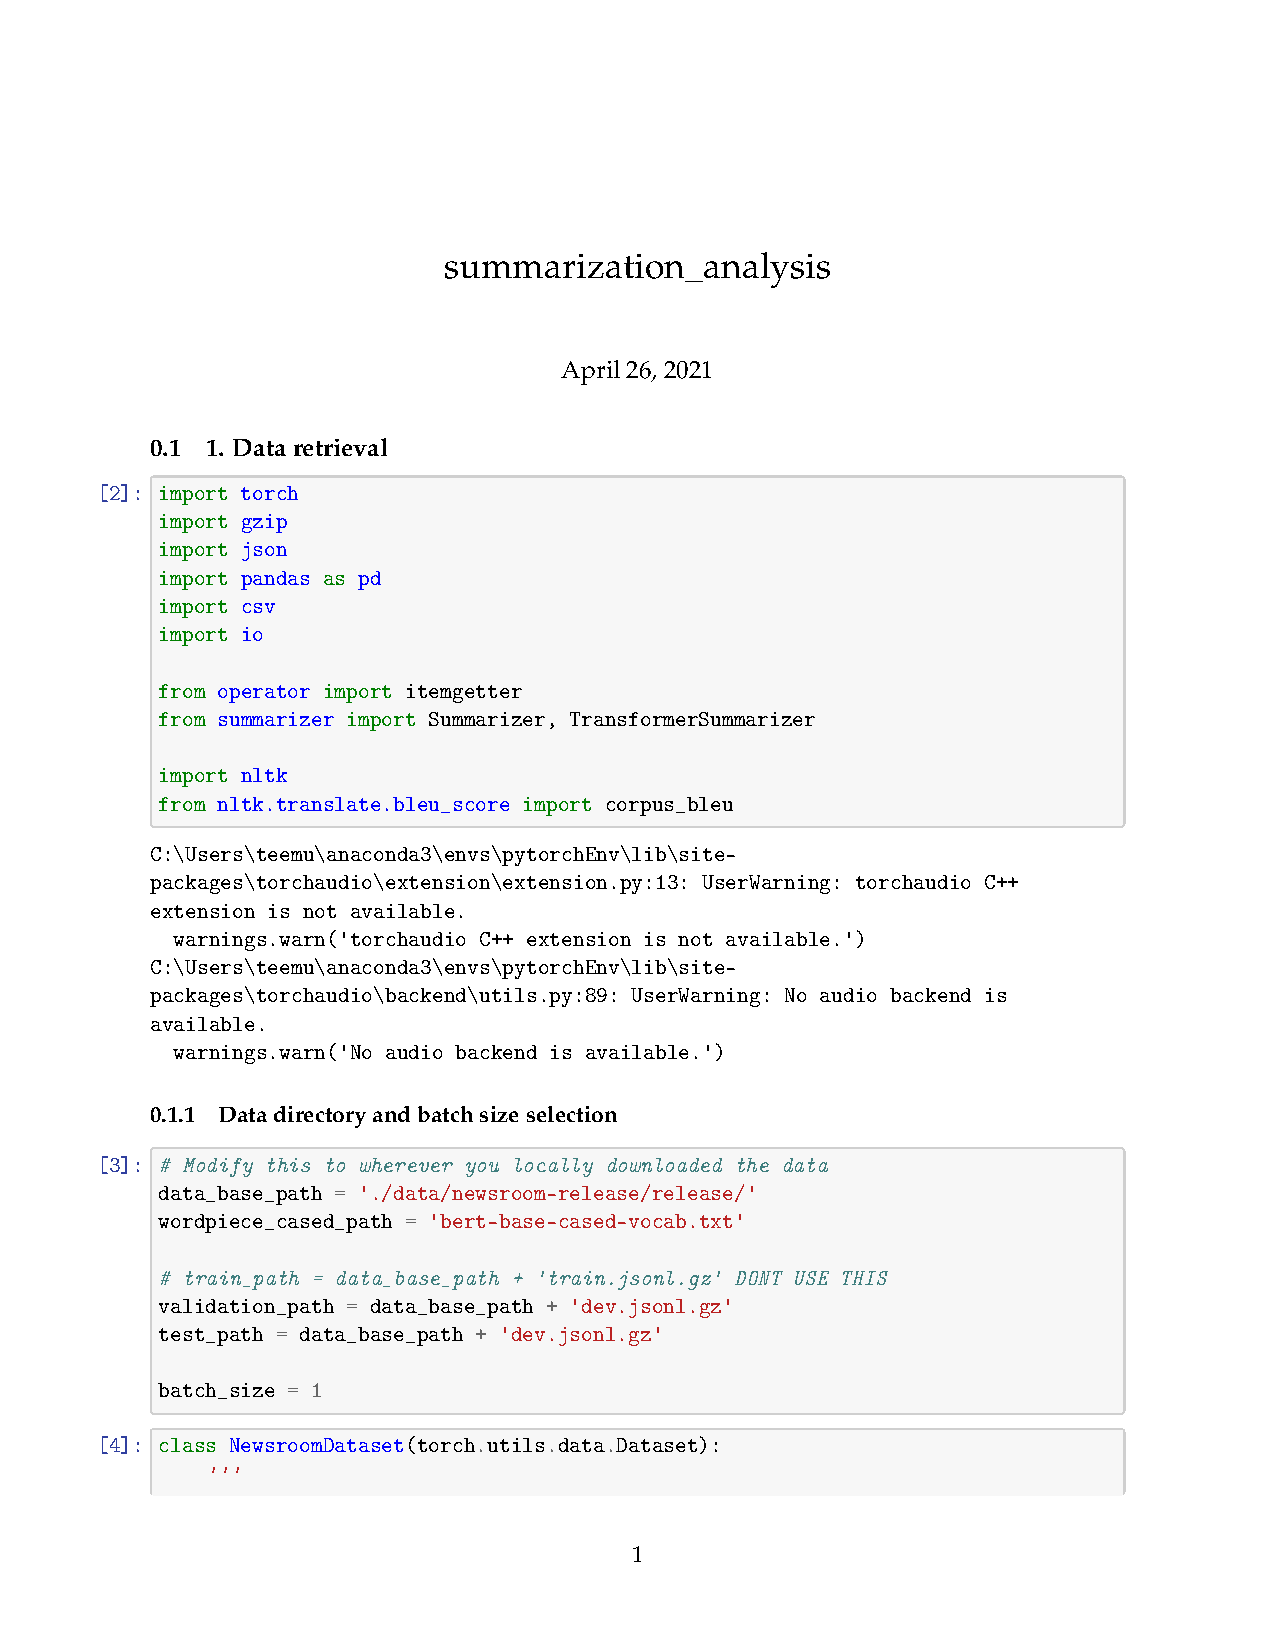
\includepdf[pages=-]{summarization_analysis}

\end{document}

